% Slide 1 ; Quels sont les contextes et les motivations de ce TER
% Slide 2 :
% Slide 3 :
% Slide 4 :

\documentclass{beamer}

\mode<presentation>
{
  \usetheme{CambridgeUS}      % or try Darmstadt, Madrid, Warsaw, ...
  \usecolortheme{dolphin} % or try albatross, beaver, crane, ...
  \usefonttheme{default}  % or try serif, structurebold, ...
  \setbeamertemplate{navigation symbols}{}
  \setbeamertemplate{caption}[numbered]
  \setbeamertemplate{itemize/enumerate subbody end}{\vspace{-0.6cm}}%
} 

\usepackage[french]{babel}
\usepackage[utf8x]{inputenc}
\usepackage{csquotes}


\title[TER]{Factorisation matricielle non-n\'egative et classification d'images}

\author[M. BEN HAMDOUNE Y. TANNIER]{Mohamed BEN HAMDOUNE \\ Yannis TANIER}

\institute[]{\bf Université Paris-Descartes}

% logo of my university
\titlegraphic{
   
\includegraphics[width=2cm]{logo}
}
\date{18 Mai 2018}

\makeatletter
\setbeamertemplate{footline}
{
  \leavevmode%
  \hbox{\fontsize{7}{7}\selectfont%
  \begin{beamercolorbox}[wd=.333333\paperwidth,ht=2.25ex,dp=1ex,center]{author in head/foot}%
    \usebeamerfont{author in head/foot}\insertshortauthor~~\beamer@ifempty{\insertshortinstitute}{}{}
  \end{beamercolorbox}%
  \begin{beamercolorbox}[wd=.333333\paperwidth,ht=2.25ex,dp=1ex,center]{title in head/foot}%
    \usebeamerfont{title in head/foot}\insertshorttitle
  \end{beamercolorbox}%
  \begin{beamercolorbox}[wd=.333333\paperwidth,ht=2.25ex,dp=1ex,right]{date in head/foot}%
    \usebeamerfont{date in head/foot}\insertshortdate{}\hspace*{1em}% original: 2ex
    \insertframenumber{} / \inserttotalframenumber\hspace*{1ex}% original: 2ex
  \end{beamercolorbox}}%
  \vskip0pt%
}
\makeatother

\setbeamerfont{footline}{size=\fontsize{10}{11}\selectfont}


\begin{document}
\begin{frame}
  \titlepage
\end{frame}

\section{Introduction}
\begin{frame}{Travail d'\'Etudes et de Recherche (TER)}

\begin{block}{Contexte et motivations}
\end{block}

\begin{figure}
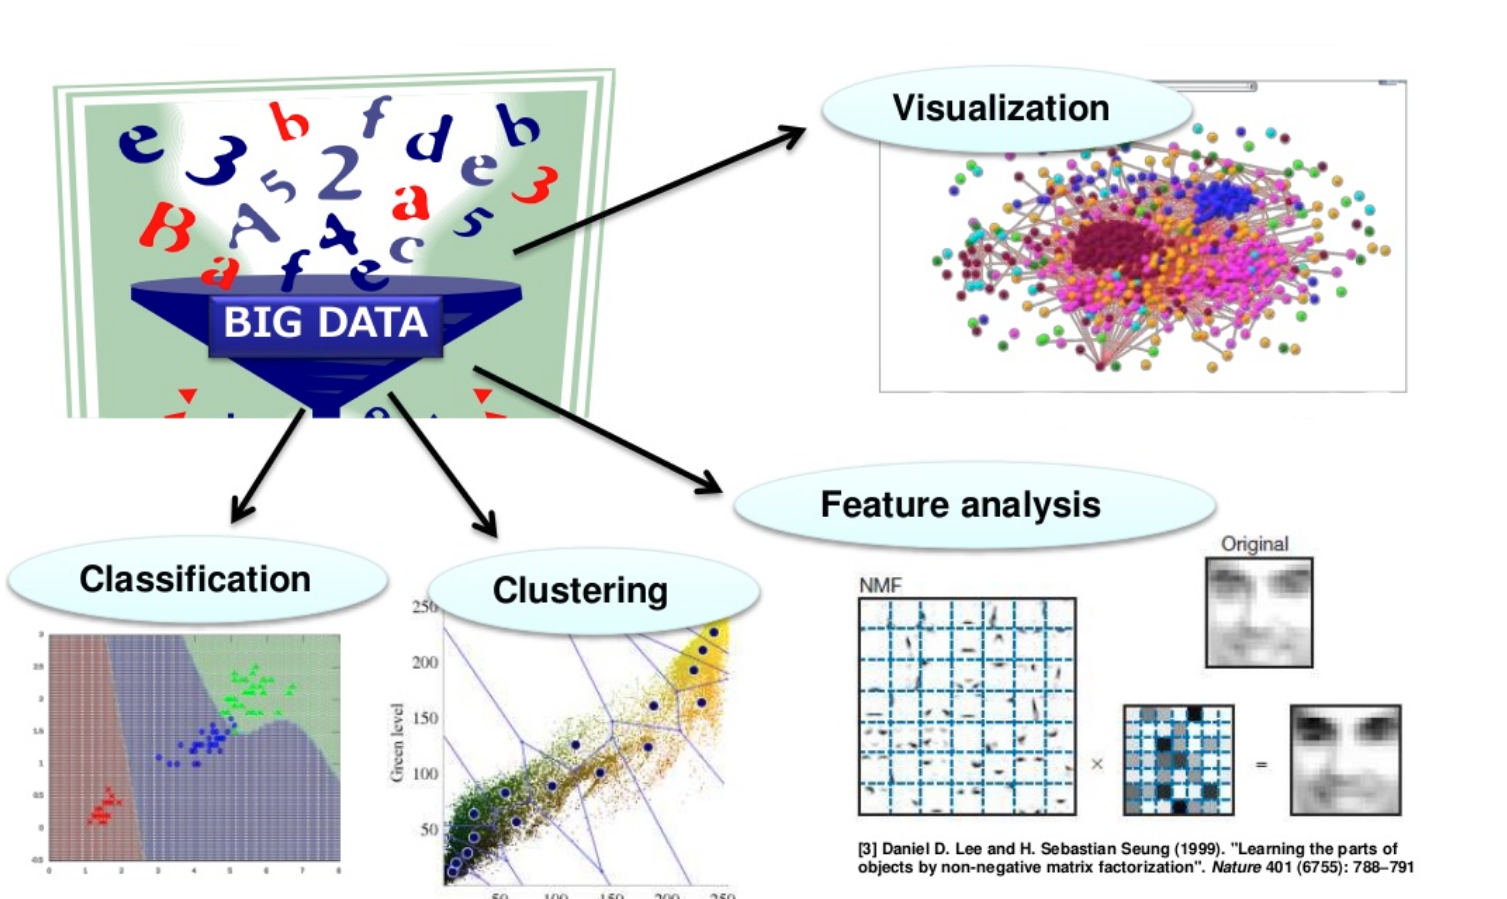
\includegraphics[width=8cm ,height= 6cm]{resume_introduction.png}
\caption{\label{fig:your-figure}Récapitulatif}
\end{figure}

\end{frame}
%%%%%%%%%%%%%%%

\section{People Art Dataset}
\begin{frame}{Jeu de données}

\begin{itemize}
  \item Présentation du jeu de données: \textbf{People-Art Dataset} .    
\end{itemize}
\begin{figure}
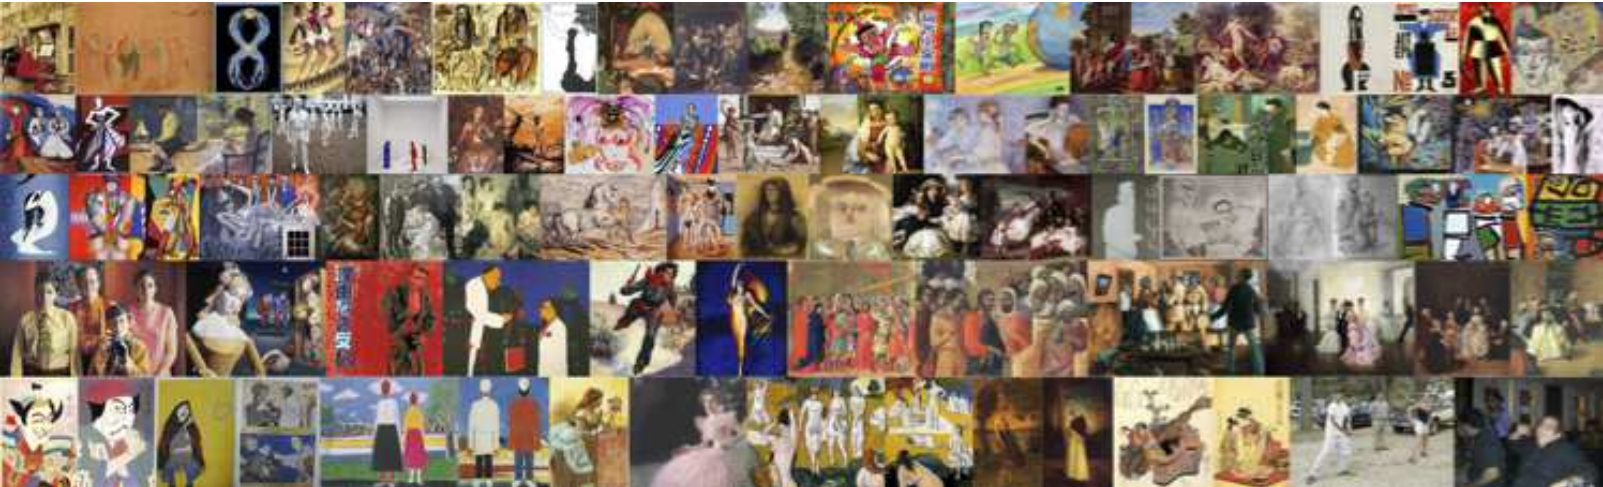
\includegraphics[width=8cm ,height= 4cm]{panel_dataset.png}
\caption{\label{fig:your-figure}\'Echantillon de People Art}
\end{figure}
\end{frame}

\section{NMF}
\begin{frame}{La factorisation matricielle non-négative}
\begin{block}{Définitions}
Soit $X \in R_+^{n\times p}$ : $X \approx WH^T$ avec $W \in R_+^{n\times k}$, $H \in R_+^{p\times k}$.    
\end{block}
\begin{block}{Points Positifs}
\begin{itemize}
  \item La contrainte de non-négativité.
  \item L'approximation par deux matrices de très faible dimensions.
  \item Les résultats sont facilement interprétables.
\end{itemize}
\end{block}
\end{frame}

\begin{frame}{La factorisation matricielle non-négative}
\begin{block}{Définitions}
Soit $X \in R_+^{n\times p}$ : $X \approx WH^T$ avec $W \in R_+^{n\times k}$, $H \in R_+^{p\times k}$.    
\end{block}
\begin{block}{Points Négatifs}
\begin{itemize}
  \item Très sensible aux bruits.
\end{itemize}
\end{block}
\end{frame}

\section{Problème d'optimisation}
\begin{frame}{Optimum Local}
\begin{block}{Fonction de perte}
L est généralement soit un critère de moindres carrés (LS ou norme de Frobenius des matrices ou "normetrace"), soit la divergence de Kullback-Leibler (KL).
\end{block}
\begin{block}{Fonction de Régularisation}
P est utilisée pour forcer les propriétés recherchées des matrices W et H, par exemple, la parcimonie des matrices ou la régularité des solutions dans le cas de données spectrales.
\end{block}
\begin{block}{Formule}
\begin{figure}
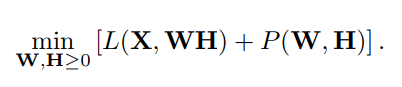
\includegraphics[width=4cm ,height= 2cm]{fonction_de_min.png}
\end{figure}
\end{block}
\end{frame}


%%%%%%%%%%%%%%%%

\section{Clustering}

\begin{frame}{Méthodes d'initialisation}

\begin{block}{ACP - Propriétés}
\begin{itemize}
  \item Les coefficients n'ont pas de contraintes.
\end{itemize}
\end{block}

\end{frame}

\begin{frame}{Méthodes d'initialisation}

\begin{block}{ACP - Propriétés}
\begin{itemize}
  \item Les coefficients n'ont pas de contraintes.
\end{itemize}
\end{block}

\begin{block}{NNDSVD - Propriétés}
\begin{itemize}
\item Unicité de la factorisation matricielle.
\end{itemize}
\end{block}


\end{frame}

\begin{frame}{Méthodes d'initialisation}
\begin{block}{ACP - Propriétés}
\begin{itemize}
  \item Les coefficients n'ont pas de contraintes.
\end{itemize}
\end{block}

\begin{block}{NNDSVD - Propriétés}
\begin{itemize}
\item Unicité de la factorisation matricielle.
\end{itemize}
\end{block}

\begin{block}{Spherical et K-Means - Propriétés}
\begin{itemize}
\item Recherche du nombre de cluster $k$ optimal.
\end{itemize}
\end{block}
\end{frame}


\begin{frame}{Algorithmes NMF}
\begin{block}{Brunet}
\begin{itemize}
  \item {Méthode Standard de NMF, basée sur la divergence de Kullback-Leibler.}
\end{itemize}
\end{block}

\begin{block}{Lsnmf}
\begin{itemize}
\item Méthode de factorisation de la matrice des moindres carrés non-négatif utilisant une méthode de gradient 
\end{itemize}
\end{block}

\begin{block}{Nsmf}
\begin{itemize}
\item Nonsmooth Non negative Matrix Factorisation
\end{itemize}
\end{block}

\begin{block}{SepNmf}
\begin{itemize}
\item Separable Nonnegative Matrix Factorization
\end{itemize}
\end{block}

\end{frame}


\section{Résultat}


\begin{frame}{Résultat}

\begin{itemize}
  \item K-means / SK-means k = 43   
\end{itemize}
\begin{figure}
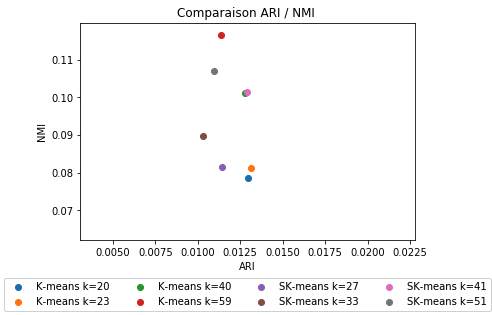
\includegraphics[width=8cm ,height= 4cm]{clustering-comparaison.png}
\end{figure}

\end{frame}

\begin{frame}{Résultat}

\begin{itemize}
  \item NMF rank = 43    
\end{itemize}
\begin{figure}
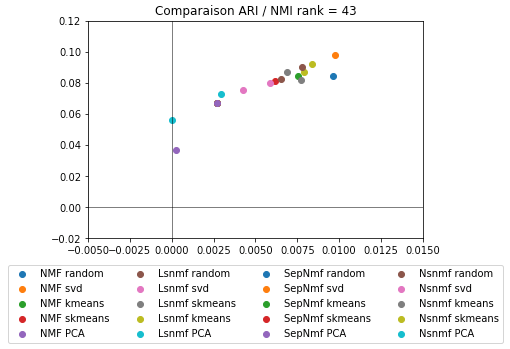
\includegraphics[width=8cm ,height= 4cm]{ari_nmi_rank43.png}
\end{figure}

\end{frame}



\begin{frame}{Clustering}
\begin{block}{K-means et Sk-means - Critères du choix nombre de cluster}
\begin{itemize}
\item Le coefficient de Silhouette
\item La méthode du Coude 
\end{itemize}
\end{block}

\begin{block}{NMF - Critères du choix du rang}
\begin{itemize}
\item Le coefficient de cophenetic
\item Le coefficient de Silhouette
\item La méthode du Coude 
\end{itemize}
\end{block}
\end{frame}




\begin{frame}{Résultat}

\begin{itemize}
  \item Comparaison des partitions
\end{itemize}
\begin{figure}
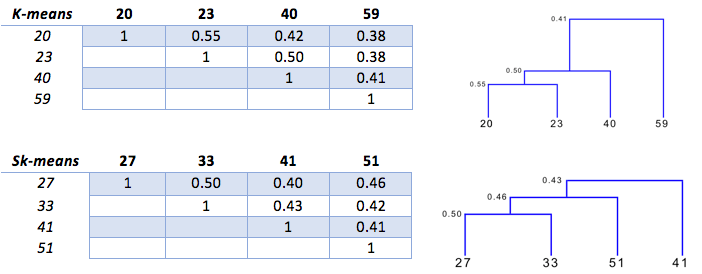
\includegraphics[width=8cm ,height= 4cm]{ari_nmi.png}
\end{figure}

\end{frame}



\begin{frame}{Résultat}

\begin{itemize}
  \item Comparaison des méthodes de la NMF
\end{itemize}
\begin{figure}
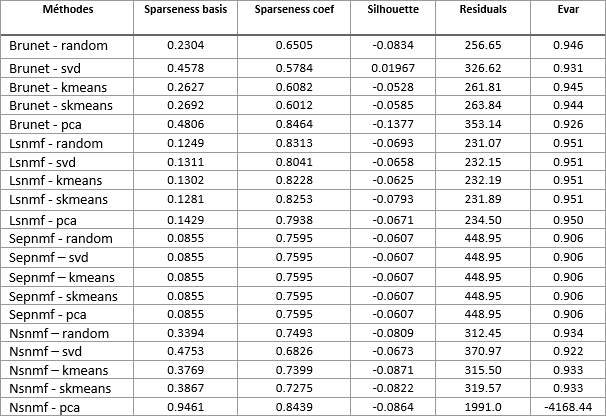
\includegraphics[width=9cm ,height= 5cm]{tab-resultat.png}
\end{figure}

\end{frame}




\begin{frame}{Résultat}

\begin{itemize}
  \item Exemple résultat partition NMF
\end{itemize}
\begin{figure}
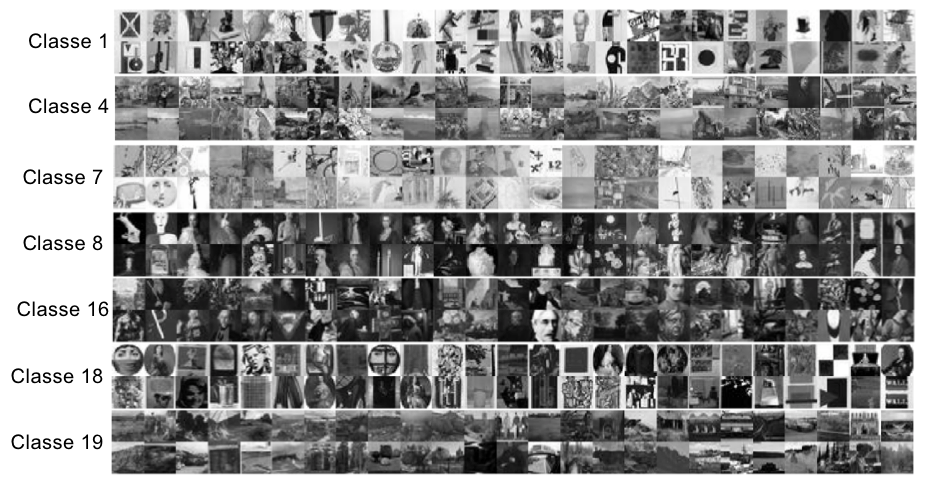
\includegraphics[width=11cm]{partition20.png}
\end{figure}

\end{frame}





\section{Conclusion}

\begin{frame}{Conclusion}
\begin{block}{Difficultés}
\begin{itemize}
\item Filtre RGB.
\item Filtre Binaire.
\item Complexité temporelle.
\end{itemize}
\end{block}
\end{frame}

\begin{frame}{Conclusion}
\begin{block}{Solutions}
\begin{itemize}
\item CNN (Réseaux de neurones convolutifs).
\item Deep NMF. 
\end{itemize}
\begin{figure}
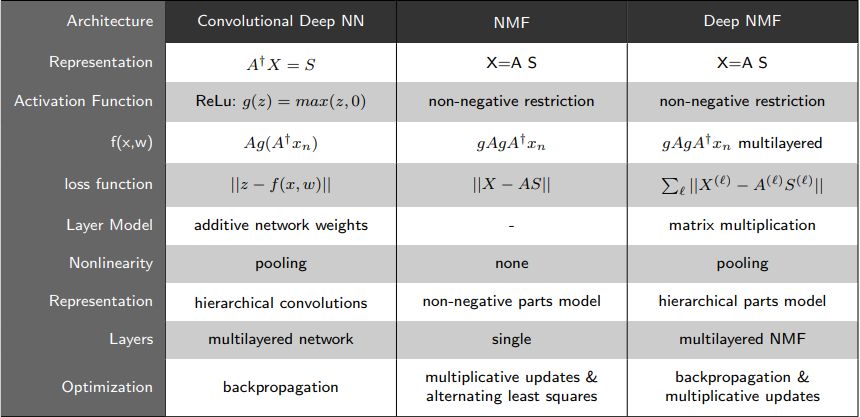
\includegraphics[width=11cm ,height= 5cm]{final_screen.png}
\caption{\label{fig:your-figure}Résumé}
\end{figure}
\end{block}

\end{frame}

%---------------------
\section{References}
\begin{frame}
\frametitle{References}
\bibliography{references} 
\bibliographystyle{ieeetr}
\begin{itemize}
\cite{Lee2001}
\cite{wild}.
\cite{nadif}.
\cite{final}.
\cite{deepnmf}.
\end{itemize}
\end{frame}

\section{Fin de la présentation}
\begin{frame}
\begin{itemize}[<+-| alert@+>]
\item Merci de votre attention.
\end{itemize}
\end{frame}

\end{document}
